\newpage
\subsection{Implementation of the embedded server}
This server can be implemented using any suitable hardware and software.
Choosed tools and libraries are not fixed and can be easily changed in
future.
Loosely coupled modules in the system give a possibility to change everything
without a need of global redesign.

The reason why technologies below are used is that they are simple to use and
easy to learn. They are also quite lightweight and therefore they can be used in
a embedded system.

\subsubsection{Hardware}
\label{sec:hardware}
\begin{center}
 \begin{figure}[h]
	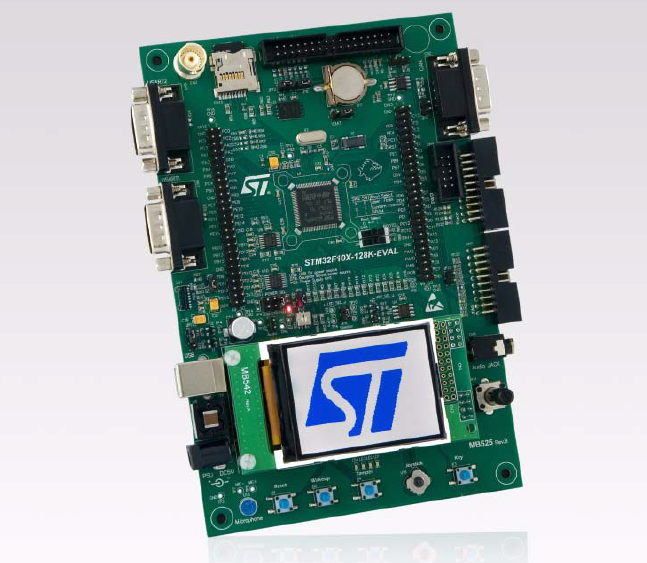
\includegraphics[width=\textwidth]{../images/implementation/embedded_server/stm3210b-eval.png}
	\caption{STM32F10X 128K evaluation board (STM3210B-EVAL)
	\cite{stm_eval_board_manual}}
	\label{fig:stm_eval_board}
 \end{figure}
\end{center}

The hardware used in this work are the two ARM Cortex M3 microcontrollers from
STMicroelectronics(\url{http://www.st.com/}). They were choosed because the
company already has a development board  and some other products from that
manufacturer. There is nothing special in that hardware and similar
microcontrollers from other manufacturers may be used in the same way.

The hardware features desribed below are common for almost all microcontrollers
and every well known manufacturer has similar device family.

Description will start from the first used STM32 microcontroller and
the STM3210B-EVAL evaluation board from STMicroelectronics.
These are features that this board has \cite{stm_eval_board_manual}:
\begin{itemize}
  \item Three 5V power supply options: power jack, USB connector or daughter
  board
  \item Boot from user Flash, test Flash or SRAM
  \item Audio play and record
  \item 64Mbyte MicroSD card
  \item Type A and Type B smartcard support
  \item 8Mbyte serial Flash
  \item I2C/SMBus compatible serial interface temperature sensor
  \item Two RS232 communication channels with support for RTS/CTS handshake on
  one channel
  \item IrDA transceiver
  \item USB 2.0 full speed connection
  \item CAN 2.0A/B compliant connection
  \item Induction motor control connector
  \item JTAG, SWD and trace tool support
  \item 240x320 TFT color LCD
  \item Joystick with 4-direction control and selector
  \item Reset, wakeup, tamper and user push buttons
  \item 4 LEDs
  \item RTC with backup battery
  \item Extension connector for daughter board or wrapping board 
\end{itemize}

As you see there are lots of opportunities to apply your creativity.
The amount of features is quite big, but we do not need most of them.
Required are only connectivity(RS232, USB) and debug(JTAG, SWD) interfaces.

This development board is made for evaluation of STM32F10x family
microcontrollers. These are ARM Cortex-M3 core-based mainstream microcontrollers
with a maximum CPU speed of 72 MHz and Flash memory amount from 16 Kbytes
to 1 Mbyte. They are equipped with large variety of peripherals.
\autoref{fig:stm32f103vbt6_hardware} covers interfaces of STM32F103VBT6 MCU that
is used in this board.

This controller is equipped with 20KB SRAM and 128KB Flash memory.
It has three USART transceivers and the debugging interface.
These are the main features we need.

\begin{center}
 \begin{figure}[h]
	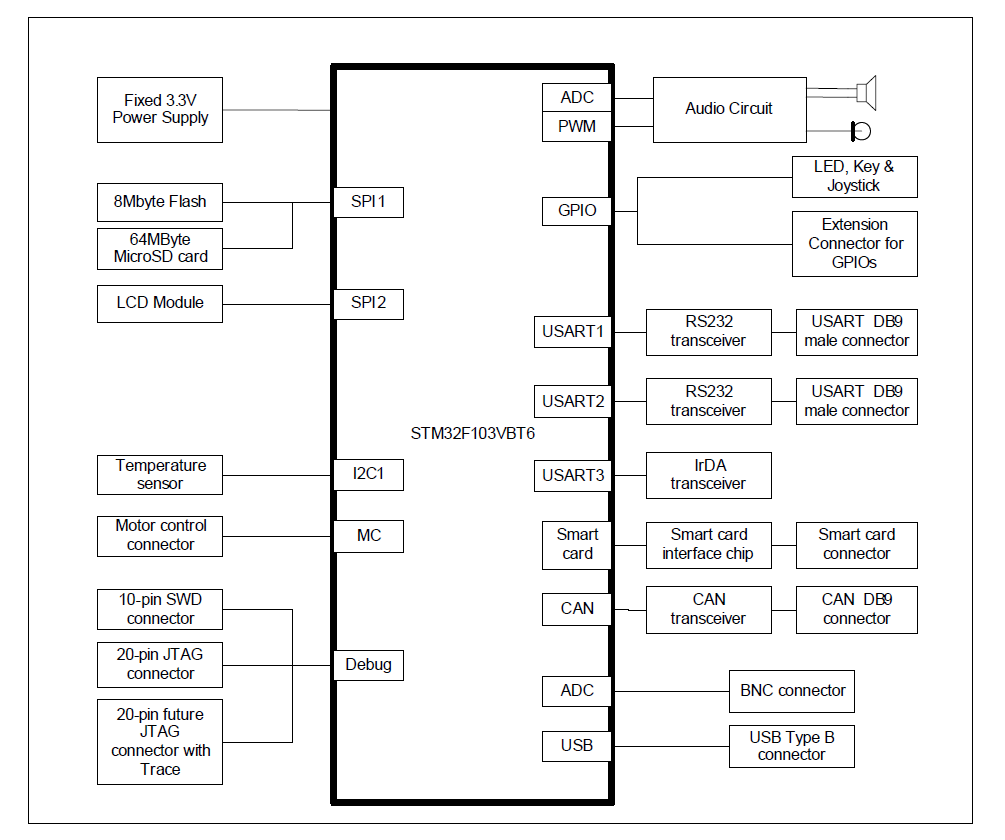
\includegraphics[width=\textwidth]{../images/implementation/embedded_server/stm32f103vbt6_hardware.png}
	\caption{Hardware block diagram of STM32F103VBT6 MCU on STM3210B-EVAL board
	\cite{stm_eval_board_manual}}
	\label{fig:stm32f103vbt6_hardware}
 \end{figure}
\end{center}

The second microcontroller that was used  is the STM32F103ZE MCU. It has more
memory:
64KB SRAM and 512KB Flash memory. This controller was choosed because the first
one has not enough resources, especially SRAM memory. The text messages, that
are transfered from client to server and back, require to be stored in the RAM
memory and each request has several copies of data while it is processed.
Amount of RAM on the first MCU was enough to execute optimized and final version of the server, but during development there is need for
storing additional debug information and to try different libraries.
The second reason is that service contracts are stored in the flash memory.
STM32F103VBT6 has 128 Kbytes of flash, however STM32F103ZE has 512 Kbytes.
System becomes more simple when service contract is stored together with
application code and there is no need to introduce another level of complexity (
connecting external storage device and programming connectivity code for
that). 


STM32F103ZE has 5 USART interfaces which is more than enough for this kind of
system. Three of them are used in the application: One for client-server
communication, one for logging and the third one for communicating with coffee
machine.

Client and server are connected using Bluetooth-to-serial module LMX9838 from
Texas Instruments.This module contains hardware and firmware support of
Bluetooth and Serial Port Profile and can be used as simple wireless serial
interface in communication between devices.

Server logging interface is connected to a personal computer using FTDI
Serial-to-USB chip (\url{http://www.ftdichip.com/}). This is popular solution of
connecting embedded systems and USB powered hardware. There is the virtual com
port on the PC side, that is powered by drivers of operating system. This
solution can be used instead of old serial connectors, that are not always
available on modern hardware.

Embedded service server and coffee machine are connected using serial line and
wires. This is a most simple connection here. Coffee machine has external serial
interface and STM32 microcontroller is connected directly to it.

That was a short overview of system hardware. Next comes description of system
software and operating system.

\subsubsection{Software and operating system}

\paragraph{Hardware configuration} ~\\
All MCU hardware is controlled by the software.
The execution of a trivial program (like "Hello world") on a
microcontroller requires a long list of instructions. To write some bytes to
UART or to blink with LED you usually need to:
\begin{enumerate}
  \item Configure MCU clock. Select clock source, frequency, clock prescalers
  \item Configure clock for peripheral buses. Again, the source and frequency by
  configuring prescalers. (Advanced Peripheral Bus in case of ARM)
  \item Turn on clocking for buses and peripherals.
  \item Configure general purpose input/output (GPIO) ports to use required
  function.
  \item Configure interrupt controller for the peripherals.
  \item In case of UART or any other communication, set the communication speed
  and configure the interface parameters.
  \item Write your application code
  \item Download the code to the device
  \item Debug the results
  \item Start from the beginning.
\end{enumerate}

Modern MCUs, especially with ARM Cortex-M architecture, have very complex
structure. They contain a huge amount of interfaces ( see \ref{sec:hardware}
section and feature list of evaluation board ) in a one single chip.
Most of peripherals are separately clocked, which gives a possibility to turn
off inactive ones and save the power energy. During MCU system startup
programmers code  should turn on and configure required peripheral modules.

In contrast, traditional software developing for desktop computers requires only
last four steps and the most complicated preparation step is the compiler and
IDE environment setup.

Each "configuring" step requires deep knowledge about what you are doing. MCU is
configured by values that are stored in memory mapped control registers. Each
register has a special purpose and different values written there configure
various MCU modules. In general words, you need to know these values to
configure the MCU system properly. Each bit in the control register represent
some setup setting.

Every controller family from various manufacturers differs from each other.
Therefore there is no need to write here in deep details how to configure one
special MCU named STM32F103ZE from STM32F1, what values to write into
\texttt{USART1->CR1} control register and which register bit turns on the UART
parity check. These instructions are not portable. When MCU hardware
changes(even families from a single manufacturer may highly differ) you need to
write this part once more.

There are two possible and more portable ways how to configure a STM32
microcontroller: Using CMSIS\footnote{The ARM® Cortex™ Microcontroller Software
Interface Standard (CMSIS) is a vendor-independent hardware abstraction layer for the Cortex-M processor series.}
from ARM and Standard Peripheral Library from STMicroelectronics. These are
hardware abstraction layer libraries that help to write portable code. They
define standard  application programming interace (API) for the ARM
architecture. Hardware vendors provide CMSIS compliant bindings for their
harware and programmers may write their code in standart manner, reducing
resources for platform change and reusing existing code.

Standard Peripheral Library is a C language library that provides standard API
for programming STM microcontrollers. It also contains CMSIS inside for
managing ARM core. There are several data structures, macros and functions that
help to configure and manage MCU peripherals.
The famous UART may be configured using Standard Peripheral Library like this:

\begin{listing}[H]
\begin{minted}[frame=lines,
               framesep=2mm]{c}
RCC_APB2PeriphClockCmd(RCC_APB2Periph_USART1, ENABLE);

USART_InitTypeDef USART_InitStructure;
USART_InitStructure.USART_BaudRate = 115200;
USART_InitStructure.USART_WordLength = USART_WordLength_8b;
USART_InitStructure.USART_StopBits = USART_StopBits_1;
USART_InitStructure.USART_Parity = USART_Parity_No;
USART_InitStructure.USART_HardwareFlowControl = USART_HardwareFlowControl_None;
USART_InitStructure.USART_Mode = USART_Mode_Rx | USART_Mode_Tx;
USART_Init(USART1, &USART_InitStructure);
\end{minted}
\caption{USART1 initialization using Standard Peripheral Library}
\label{lst:uart_init_example}
\end{listing} 

Most of configuration can be done using preprocessor defines.
You may add several defines, for example \texttt{#define STM32F10X_MD} to use
STM32 Medium density devices (Flash memory density ranges between 64 and 128
Kbytes). Clock rates and different peripherals can be adjusted in a similar way.

The distibution of STM Standard Peripheral Library contains a lot of
code and application examples, that helped me a lot. I have found there how to
configure a USART DMA\footnote{Direct Memory Access} controller and how to
transfer bytes using USART without intervention of central processing unit.
This is  quite good source for the begginers like me.

Setup an embedded development environment takes a lot of time and requires
deep knowledge about the underlying hardware. It is good to have such tools like
standart APIs, that help to make this process more easy.

\paragraph{Operating system}



\subsubsection{Service software}
Here will be STM32 server implementation.







%  One solution is to use closed encrypted proprietary
% protocol and be calm, but as it was mentioned earlier, it limits the possibility of integration
% between other embedded systems. It this case all of your devices should support
% that protocol and you choise of different hardware is limited. Proprietary
% protocols are often vendor-specific, code is closed, documentation is not free
% and all it works only with the proprietary devices from the manufacturer.
% 
% 
% \begin{center}
%  \begin{figure}[h]
% 	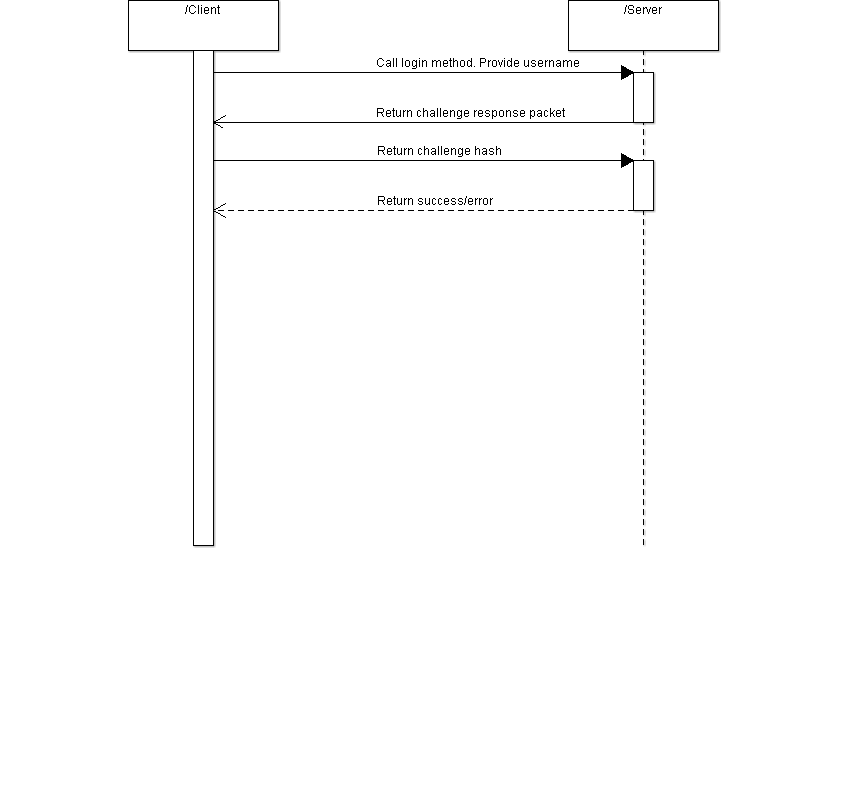
\includegraphics[width=\textwidth]{../images/implementation/embedded_server/SequenceDiagram.png}
% 	\caption{Client authentification process}
% 	\label{fig:embedded_server_login_auth}
%  \end{figure}
% \end{center}

%reversably encrypted form.

